\documentclass{article}
\IfFileExists{TeXmacs.sty}
  {\usepackage{TeXmacs}}
  {\usepackage{/usr/share/TeXmacs-1.0.0.6/misc/latex/TeXmacs}}
\newcommand{\chapter}[1]{\tmsection{\begin{center}\huge #1\end{center}}}

\begin{document}

\title{Giac/Xcas}\author{B. Parisse, R. De Graeve}\maketitle

Giac is a C++ library for computer algebra system computation. Xcas is a
graphical interface to Giac that run on many platforms including Windows,
GNU/Linux (PC and PDA like the HP iPaq with the Familiar distribution or the
Sharp Zaurus with Xfree86), Mac OS X. The main features of Xcas are:
\begin{enumeratenumeric}
  \item The usual features of a graphical calculator (including a programming
  language)
  
  \item Symbolic mathematical functions (expand/factor,
  derivation/integration, solvers,...)
  
  \item An equation editor
  
  \item Interactive geometry
  
  \item A small spreadsheet
  
  \item On-line help
\end{enumeratenumeric}


In the first section, we present the interface of xcas, in the second section
we give technical data about Xcas (memory requirements, ...).

\section{Xcas interface}

The xcas window is divided in 2 parts horizontally: the left part contains the
software output, the right part is the keyboard of the virtual calculator.

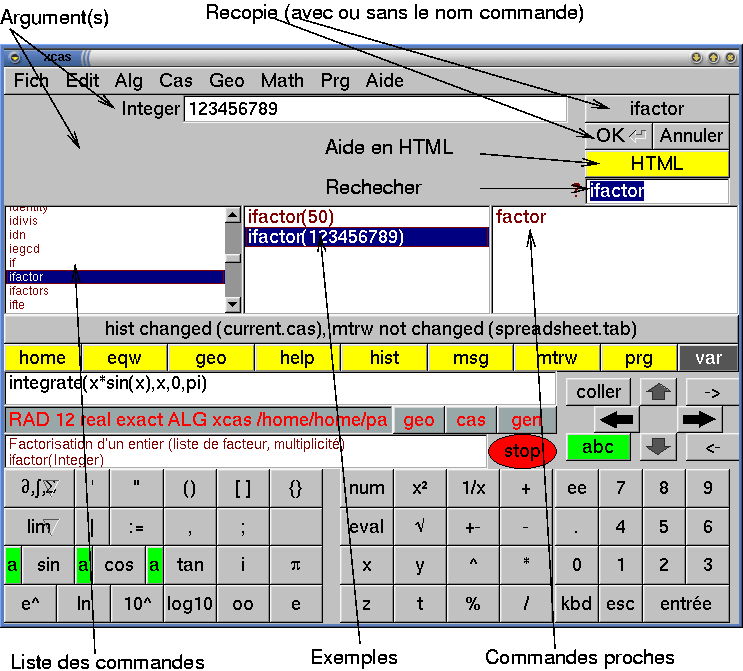
\epsfig{file=xcas1.eps}

The left part is composed of
\begin{enumeratenumeric}
  \item The menu bar.
  
  \item The view area. It is occupied by the history or geometric or program
  or equation or matrix view.
  
  \item Buttons specific to the current view (here history navigation
  buttons).
  
  \item The input line (or commandline).
  
  \item The soft menu buttons giving quick access to the menu bar option and
  the yellow buttons to change the view.
  
  \item The state of the calculator (here radian, 12 digits, etc.) and buttons
  to modify this state.
  
  \item The on-line help (with a browser listing all commands, the help on the
  current command, examples and related commands). Currently available in
  English, French and Spanish (here in French)
\end{enumeratenumeric}
Beginners can choose a function in the menu bar, e.g. Cas->Calc->integrate,
click on the first example, modify it to suit their needs and press the enter
key or button.

The geometry view is switched on by clicking on the yellow geo key or by
issuing any graphical command like Math->Graph->plotfunc to represent a
function. Commands in the inputline are evaluated like in the history view. In
addition clicking on the geometric area will draw a point, and
push-drag-release will draw a segment. We show an example of a triangle ABC
with the circle ABC in the same plot as the graph of the function $x -
\frac{1}{6} x^3$ (we have switched on-line help language to English)

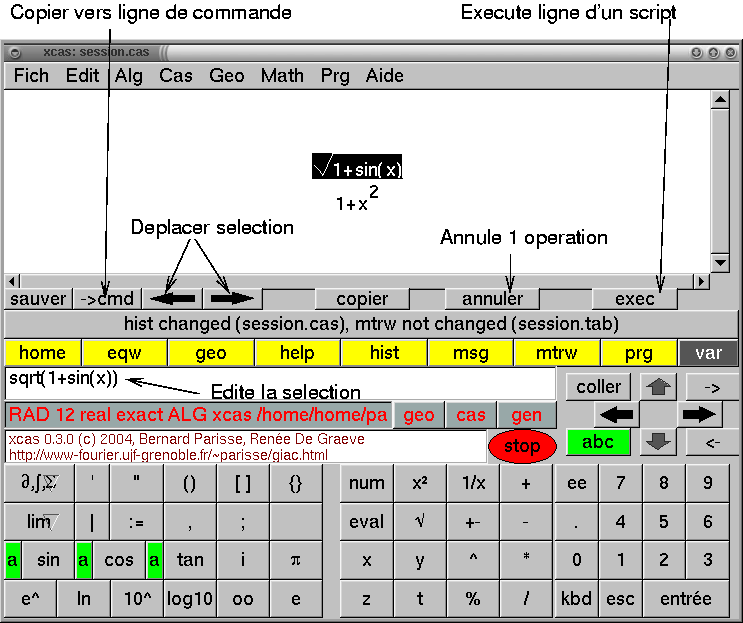
\epsfig{file=xcas2.eps}

Like with other interactive geometry package, one can move the point A, B or C
and the whole figure will dynamically move. But unlike other geometry package
it is possible to define the geometric objects with exact coordinates and make
proof of geometric properties with the symbolic engine instead of numerical
checks.

The program view (yellow prg button) gives access to a small program editor,
we show here as an example how to compute the greatest common denominator of
two integers using Euclide algorithm, an universal example to teach the basic
of algorithmic.

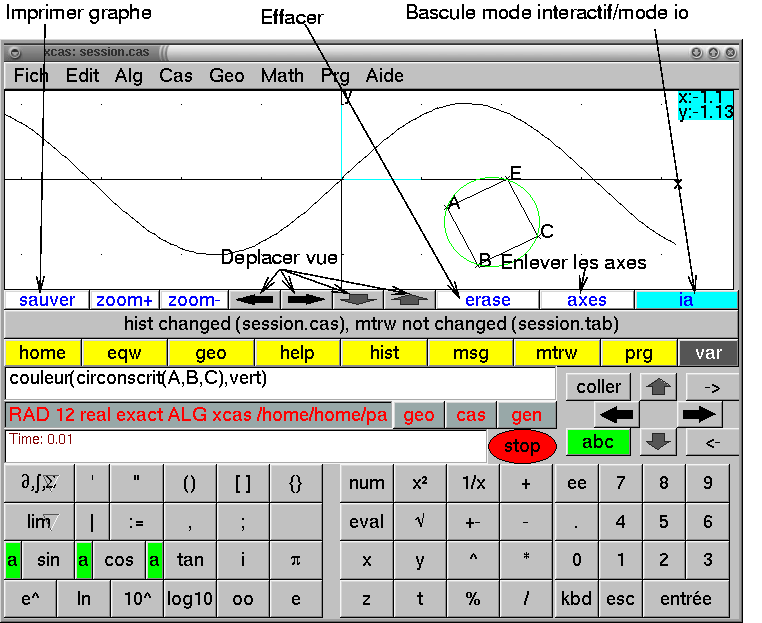
\epsfig{file=xcas3.eps}

The syntax can be choosed similar to C, or Maple or Mupad. There is an
interactive debugger to help correcting runtime errors.

The eqw view gives access to a powerful way to edit mathematical expressions
using the symbolic engine behind to perform simplifications on subexpressions.

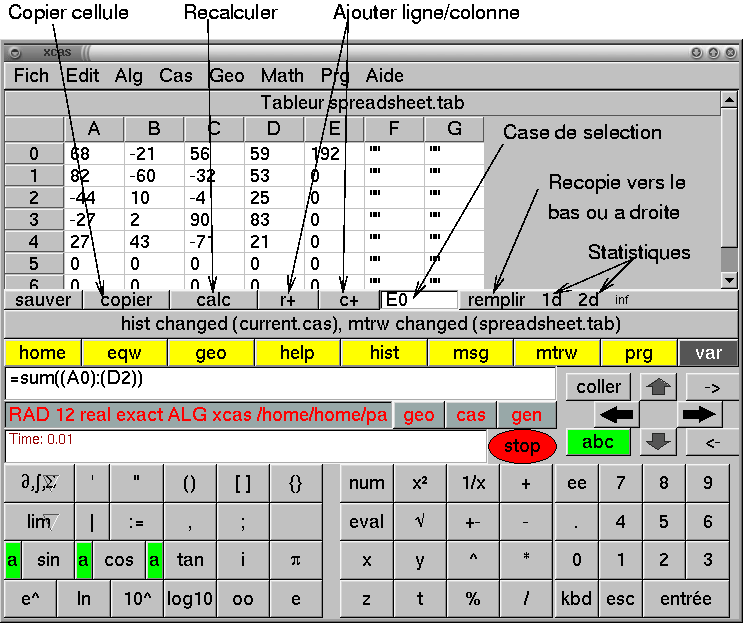
\epsfig{file=xcas4.eps}

The last view is the matrix view that gives an easy way to enter a matrix and
as also some spreadsheet functionnalities (absolute, relative cells, the cell
content can be a symbolic expression, the programming language can be used to
define one cell as a function of other cells).

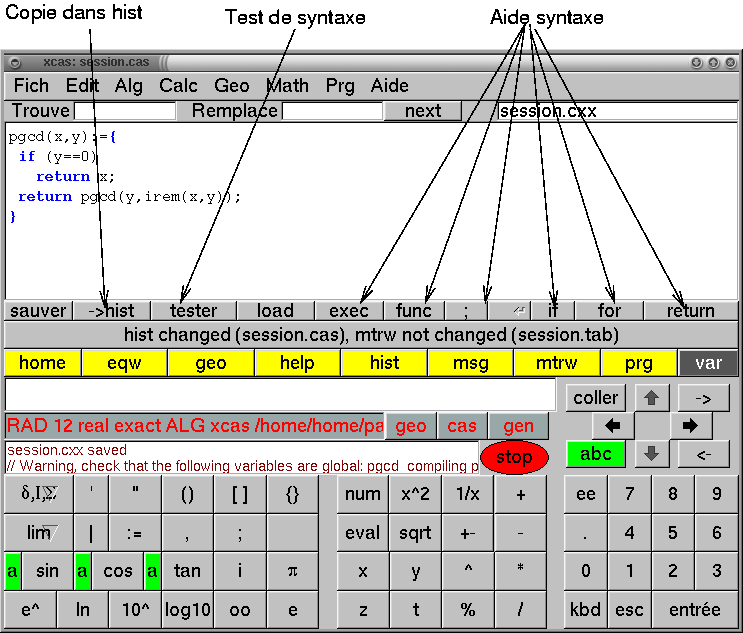
\epsfig{file=xcas5.eps}

In the example above we use the spreadsheet to return the table of value of
the sin function starting from -6 with a step of 1.2. It is fairly easy to
change the function (edit cell B0), the init value (cell A1) or the step (cell
B1).

Configuration is done with choosebox or for the language localization using
the menu.

In conclusion, xcas has the features corresponding to the mathematical
curriculum of highschool and university. The same software runs on ARM PDA
with linux, PC with Windows or Linux and on the Mac making data exchange easy.

\section{Requirements}

Giac the C++ library is licensed under the GPL (dual-licensing might be
possible). It requires the GMP (Gnu Math Precision library, LGPL).
Optionnally:
\begin{enumerateroman}
  \item Advanced numeric functions (like matrix factorizations) requires the
  GSL (Gnu Scientific Library, GPL).
  
  \item Advanced number-theoritic functions require the PARI library (GPL)
  
  \item Advanced polynomial factorization is faster with the NTL library
  (GPL).
\end{enumerateroman}
The source code is about 60,000 lines of code.

The xcas interface is built over FLTK and, for the spreadsheet, FLVW. The code
is about 10,000 lines.

Compilation requires a C++ compiler compliant with ANSI-3, like g++ 2.95 and
above. Compilation for the ARM Linux platform is as easy as for the x86
platform.

Compiled statically with GSL, without PARI/NTL, xcas is around 5Mo and 1.3Mo
on a compressed filesystem (like jffs2 on the HP iPaq familiar distribution).
The static binary requires the X-Windows system on Unix or nano-X (using flnx
instead of fltk, not tested). It runs without any problem on my iPaq (16M
flash ROM, 32M RAM, no extension card).

If xcas is compiled dynamically, it is possible to insert during a session
dynamic modules (i.e. shared libraries adding functionnalities). This can be
used for example to customize the programming language, e.g. add French or
Spanish keywords instead of if, for, while, ... It may also be used to insert
a TI89 or Maple compatibility module if/when available.

Status of the project is alpha. Roadmap: a beta version for the end of year
2002, version 1 Spring 2003.

Downloads of the binaries, source, other informations and complete French
documentation are available at:
\begin{verbatim}
http://www-fourier.ujf-grenoble.fr/~parisse/giac.html
\end{verbatim}


\end{document}
